\documentclass[12pt]{article}

% Layout.
\usepackage[top=1.2in, bottom=0.75in, left=1in, right=1in, headheight=1.0in, headsep=0pt]{geometry}

% Fonts.
\usepackage{mathptmx}
\usepackage[scaled=0.86]{helvet}
\renewcommand{\emph}[1]{\textsf{\textbf{#1}}}

% TiKZ.
\usepackage{tikz, pgfplots}
\usetikzlibrary{calc}
\pgfplotsset{my style/.append style={axis x line=middle, axis y line=middle, xlabel={$x$}, ylabel={$y$}}}
\pgfplotsset{compat=1.16}

% Misc packages.
\usepackage{amsmath,amssymb,latexsym,bm,array,multicol,enumitem}
\usepackage{graphicx}
\usepackage{xcolor}

% Commands to set various header/footer components.
\makeatletter
\def\doctitle#1{\gdef\@doctitle{#1}}
\doctitle{Use {\tt\textbackslash doctitle\{MY LABEL\}}.}
\def\docdate#1{\gdef\@docdate{#1}}
\docdate{Use {\tt\textbackslash docdate\{MY DATE\}}.}
\def\doccourse#1{\gdef\@doccourse{#1}}
\let\@doccourse\@empty
\def\docscoring#1{\gdef\@docscoring{#1}}
\let\@docscoring\@empty
\def\docversion#1{\gdef\@docversion{#1}}
\let\@docversion\@empty
\makeatother

% Headers and footers layout.
\makeatletter
\usepackage{fancyhdr}
\pagestyle{fancy}
\fancyhf{} % Clears all headers/footers.
\lhead{\emph{\@doctitle\hfill\@docdate} \medskip
\ifnum \value{page} > 1\relax\else\\
\emph{Name: \rule{3.5in}{1pt}\hfill \@docscoring}
\fi}

\rfoot{\emph{\@docversion}}
\lfoot{\emph{\@doccourse}}
\cfoot{\emph{\thepage}}
\renewcommand{\headrulewidth}{0pt}%
\makeatother

% Paragraph spacing
\parindent 0pt
\parskip 6pt plus 1pt

% A problem is a section-like command. Use \problem{5} for a problem worth 5 points.
\newcounter{probcount}
\newcounter{subprobcount}
\setcounter{probcount}{0}

\newcommand{\problem}[1]{%
\par
\addvspace{4pt}%
\setcounter{subprobcount}{0}%
\stepcounter{probcount}%
\makebox[0pt][r]{\emph{\arabic{probcount}.}\hskip1ex}\emph{[#1 points]}\hskip1ex}

\newcommand{\thesubproblem}{\emph{\alph{subprobcount}.}}

% Subproblems are an enumerate-like environment with a consistent
% numbering scheme.  Use \begin{subproblems}\item...\item...\end{subproblems}
\newenvironment{subproblems}{%
\begin{enumerate}[itemindent=8pt,leftmargin=0pt]%
\setcounter{enumi}{\value{subprobcount}}%
\renewcommand{\labelenumi}{\emph{\textsl{\alph{enumi})}} \,}%
}%
{%
\setcounter{subprobcount}{\value{enumi}}%
\end{enumerate}%
}

% Blanks for answers in normal and math mode.
\newcommand{\blank}[1]{\rule{#1}{0.75pt}}
\newcommand{\mblank}[1]{\underline{\hspace{#1}}}
\def\emptybox(#1,#2){\framebox{\parbox[c][#2]{#1}{\rule{0pt}{0pt}}}}

% Misc.
\renewcommand{\d}{\displaystyle}
\newcommand{\ds}{\displaystyle}
\newcommand{\threeopts}{{\small \hspace{-6mm} $\begin{matrix} \text{\textsc{converges}} \\ \text{\textsc{absolutely}} \end{matrix}$ \qquad\qquad $\begin{matrix} \text{\textsc{converges}} \\ \text{\textsc{conditionally}} \end{matrix}$ \qquad\qquad \textsc{diverges}} \bigskip}

\newcommand{\ba}{\mathbf{a}}
\newcommand{\bb}{\mathbf{b}}
\newcommand{\bc}{\mathbf{c}}
\newcommand{\bi}{\mathbf{i}}
\newcommand{\bj}{\mathbf{j}}
\newcommand{\bk}{\mathbf{k}}
\newcommand{\bn}{\mathbf{n}}
\newcommand{\br}{\mathbf{r}}
\newcommand{\bu}{\mathbf{u}}
\newcommand{\bv}{\mathbf{v}}
\newcommand{\bw}{\mathbf{w}}

\newcommand{\bT}{\mathbf{T}}

\newcommand{\grad}{\nabla}
\newcommand{\Div}{\nabla\cdot}

\newcommand{\ip}[2]{\mathrm{\left<#1,#2\right>}}
\newcommand{\vv}[2]{\mathrm{\left<#1,#2\right>}}
\newcommand{\vvv}[3]{\mathrm{\left<#1,#2,#3\right>}}


\newcommand{\boxy}[1]{\fbox{\Huge \strut \hspace{#1mm} \strut}}
\newcommand{\boxycontent}[2]{\fbox{\quad {\large #2} {\Huge \strut \hspace{#1mm} \strut}}}



\doctitle{\hspace{-6mm} Math 302 Differential Equations: \,{\large Quiz 5}}
\docdate{15 November 2023}
\doccourse{}
\docversion{}
\docscoring{\fbox{{\LARGE \strut}\hspace{0.8in} / 25}}


\begin{document}
$\boxed{30}$ minutes maximum.  No aids (book, calculator, etc.) are permitted.  Show all work; use proper notation for full credit.  Answers should be in reasonably-simplified form.  25 points possible.

% like 6.1 #7 on homework, but simplified
\problem{5}  Find the radius and interval of convergence of the power series \quad$\ds \sum_{k=1}^\infty \frac{(3x-1)^k}{k}$
\vfill
\hfill\boxycontent{39}{$R=$}

\hfill\boxycontent{40}{$I=$}

% like 6.2 #1 on homework
\problem{4}  What is the (minimum) radius of convergence of the power series solution of the following differential equation, about the ordinary point $x_0=0$?  Explain briefly.

\noindent (\textsl{Hint.  Do not find the series solution itself!})

\medskip
{\large $\ds (x^2-25) y'' + y' + x y = 0$}
\vspace{2.0in}

\hfill\boxycontent{39}{$R=$}

\clearpage\newpage
% like 6.1 #33 on homework but simpler
\problem{8}  Verify by direct substitution that the given power series is a solution of the differential equation.

{\large $\ds y = \sum_{n=0}^\infty \frac{(-1)^n 2^n x^n}{n!}$, \qquad $\ds y' + 2 y = 0$}
\vfill


\clearpage\newpage
% like 6.2 #21 on homework, but simpler
\problem{8}  Solve the initial value problem below by starting with a power series
    $$y(x) = c_0 + c_1 x + c_2 x^2 + \dots = \sum_{n=0}^\infty c_n x^n$$
(\textsl{Hints.  You can use summation notation or not.  Find at least the first five coefficients.  You can check your answer by non-series methods, but full credit requires a valid series calculation.})

\medskip
{\large $\ds y'' + 4 y = 0$, \qquad $\ds y(0)=3, \quad y'(0)=0$}
\vfill


\clearpage\newpage
% like 5.3 Problem 3
\noindent \emph{Extra Credit. [2 points]} \, The energy function associated to a conservative physical system is $E(x,x')=\frac{m}{2} (x')^2 + P(x)$ where $P(x)$ is the potential energy.  The negative derivative of the potential energy is the force: $P'(x) = -F(x)$.  What is the energy for the undamped, nonlinear mass-spring system with equation \quad $\ds m\, x'' = - \frac{k x}{1+x^2}$\,? \, (\textsl{Assume $m,k$ are positive constants.})
\vfill
\hfill\boxycontent{90}{$E(x,x')=$}

%\centerline{\footnotesize \textsc{extra space}}

\noindent \hrule
\medskip
\hfill 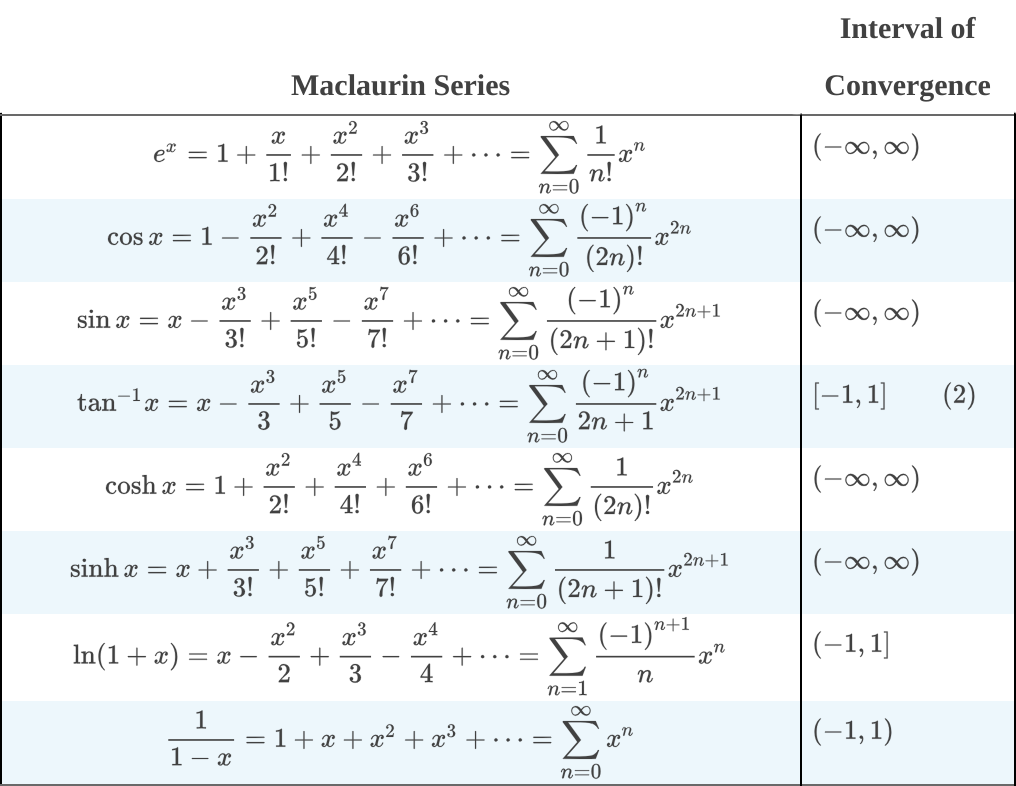
\includegraphics[width=0.55\textwidth]{figs/familiarseries.png}
\vfill
\end{document}
